\section{Lensing and joint scalar metric observables}\label{sec:lensing}

\subsection{Deflection, convergence, shear, and mass maps}
For an isotropic weak-field metric in Newtonian gauge,
\begin{equation}
\dd s^2=-(1+2\Psi/c^2)c^2\dd t^2+a^2(1-2\Phi/c^2)\dd\mathbf x^2,
\end{equation}
the lensing potential probes $(\Phi+\Psi)/2$. The matter-to-metric response specifies both potentials and their gravitational slip $\eta=\Phi/\Psi$. When the standard weak-field limit holds, the thin-lens relations are
\begin{align}
\bm\alpha(\bm\theta)&=\frac{1}{c^2}\frac{D_{ls}}{D_s}\int\nabla_\perp(\Phi+\Psi)\,\dd\ell,\\
\kappa(\bm\theta)&=\frac12\nabla_\theta^2\psi(\bm\theta)=\frac{\Sigma_{\rm mass}}{\Sigma_{\rm crit}},\qquad
\Sigma_{\rm crit}=\frac{c^2}{4\pi G}\frac{D_s}{D_lD_{ls}},\\
\gamma_1&=\tfrac12(\psi_{,11}-\psi_{,22}),\qquad \gamma_2=\psi_{,12}.
\end{align}
Here $\Sigma_{\rm mass}$ denotes projected mass per area; the dimensionless response $\Sigma$ is defined in Section~\ref{sec:metric-scalar-joint}. For $\Phi=\Psi$, integration along a straight ray gives the physical point-mass bending angle $4GM/(bc^2)$. The reduced angular deflection $\bm\alpha$ includes the additional distance ratio $D_{ls}/D_s$. The angular and surface-density conventions are fixed in the source code.

\subsection{Galaxy strong lens and time delay}\label{sec:sis}
For a singular isothermal sphere with line-of-sight velocity dispersion $\sigma_v$,
\begin{equation}
\theta_E=4\pi\left(\frac{\sigma_v}{c}\right)^2\frac{D_{ls}}{D_s},\quad
\kappa(\theta)=\gamma_t(\theta)=\frac{\theta_E}{2\theta}.
\end{equation}
The arrival-time surface gives $\Delta t=(1+z_l)(D_lD_s/cD_{ls})\,\Delta[\frac12|\bm\theta-\bm\beta|^2-\psi(\bm\theta)]$. For $z_l=0.3$, $z_s=1$, $\sigma_v=220$ km s$^{-1}$ and $\beta=\theta_E/2$, the reference geometry yields
\begin{equation}
\boxed{\theta_E=0.8884\ \mathrm{arcsec},\qquad |\Delta t|=42.93\ \mathrm{days}.}
\end{equation}
The source offset and velocity dispersion are chosen examples. The values are conditional on this lens geometry, dispersion and source position.

\subsection{Cluster lens, convergence map, and statistical shear}\label{sec:cluster-lensing}
Take a Navarro--Frenk--White density profile \cite{NFW}, $\rho(r)=\rho_s/[ (r/r_s)(1+r/r_s)^2 ]$, with $M_{200}=10^{14}\msun$, concentration $c_{200}=5$, and lens/source redshifts as above. The reference calculation gives $r_{200}=0.8826$ Mpc, and at projected radius $R=0.1$ Mpc,
\begin{equation}
\boxed{\kappa(0.1\,\Mp)=0.1197,\qquad\gamma_t(0.1\,\Mp)=0.0708.}
\end{equation}
An idealized $10^{15}\msun$ NFW cluster with $c_{200}=4$ has a tangential critical radius $R_t=0.02469$ Mpc, corresponding to $\theta_t=5.35$ arcsec for this geometry, under the adopted spherical profile and background. This last quantity is profile-dependent.

\begin{figure}[t]\centering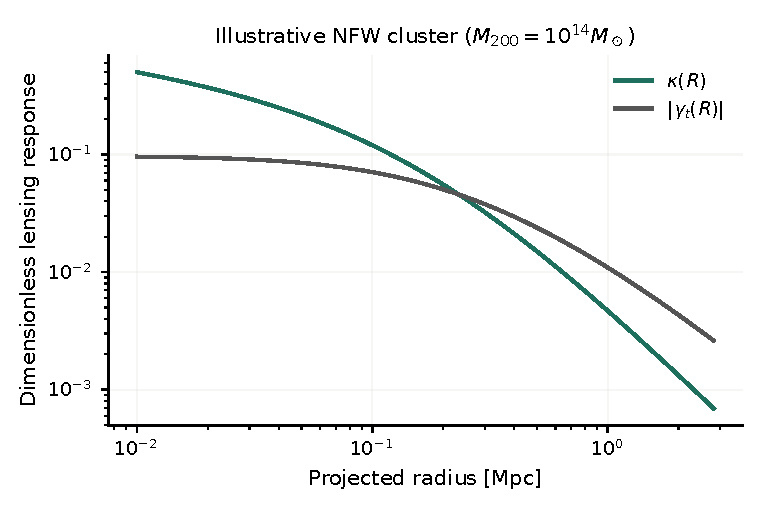
\includegraphics[width=.75\linewidth]{figures/cluster_lensing_reference.pdf}\caption{Spherically averaged NFW lens convergence and tangential shear for the stated analytic reference cluster.}\end{figure}

\begin{figure}[t]\centering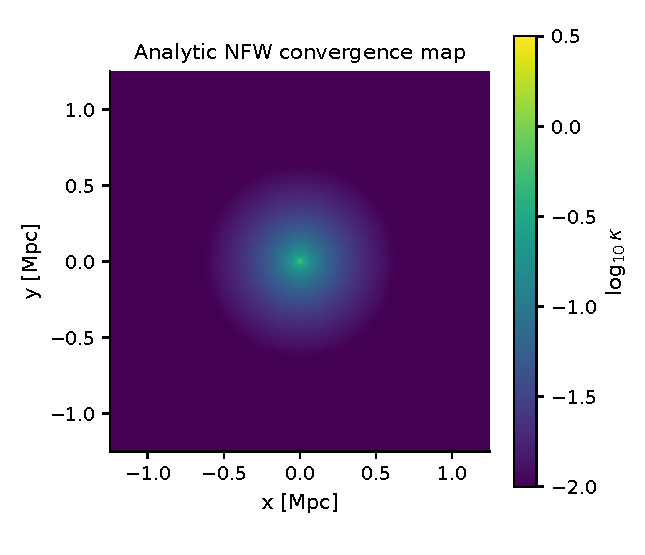
\includegraphics[width=.67\linewidth]{figures/cluster_kappa_map.pdf}\caption{Projected NFW convergence map computed analytically. The map is the projection of the specified spherical analytic density profile.}\end{figure}

For normalized comoving source distributions $n_i(\chi_s)$, define the Weyl-potential lensing efficiency
\begin{equation}
q_i(\chi)=\int_\chi^{\chi_H}\dd\chi_s\,n_i(\chi_s)\frac{\chi_s-\chi}{\chi_s\chi},
\qquad \int_0^{\chi_H}n_i(\chi_s)\,\dd\chi_s=1.
\end{equation}
Writing $P_{\Phi+\Psi}$ for the three-dimensional power spectrum of the \emph{dimensional} sum of the two Newtonian-gauge potentials, the Born--Limber angular convergence spectrum is
\begin{equation}\label{eq:weyl-limber-corrected}
C_\ell^{\kappa_i\kappa_j}\simeq \frac{[\ell(\ell+1)]^2}{4c^4}
\int_0^{\chi_H}\frac{\dd\chi}{\chi^2}\,q_i(\chi)q_j(\chi)
P_{\Phi+\Psi}\!\left(\frac{\ell+1/2}{\chi},z(\chi)\right).
\end{equation}
The angular-derivative factor and powers of $c$ are essential when the spectrum is defined for the dimensional Weyl potentials rather than the matter density. For $\Phi=\Psi$ and the standard Poisson equation, its large-$\ell$ limit agrees with the matter-spectrum convergence integral in Eq.~\eqref{eq:clkk}. A survey comparison additionally includes calibrated redshift distributions, intrinsic alignments, baryonic and nonlinear effects, masks, selection functions, and covariance.

\subsection{A computed angular convergence spectrum}
\label{sec:shear}
The standard weak-lensing limit gives a tractable \emph{angular} statistic in addition to the analytic galaxy and cluster lenses calculated above. For a thin source plane at comoving distance $\chi_s$, the first-order convergence kernel in flat GR is
\begin{equation}
W_\kappa(\chi)=\frac{3\Om_mH_0^2}{2c^2}\frac{\chi}{a(\chi)}\frac{\chi_s-\chi}{\chi_s},\qquad 0<\chi<\chi_s.
\end{equation}
Under the Born approximation and Limber correspondence $k=(\ell+1/2)/\chi$, the E-mode convergence power is
\begin{equation}\label{eq:clkk}
\boxed{C_\ell^{\kappa\kappa}=\int_0^{\chi_s}\frac{\dd\chi}{\chi^2}\,W_\kappa^2(\chi)P_\delta\!\left(\frac{\ell+1/2}{\chi},z(\chi)\right).}
\end{equation}
For a reference source redshift $z_s=1$, smooth BBKS matter transfer, observed $\sigma_8$ normalization and the linear growth solution in Section~\ref{sec:structure}, direct quadrature gives:
\begin{equation}\label{eq:numshear}
\boxed{C_{50}^{\kappa\kappa}=1.701\times10^{-8},\quad
C_{200}^{\kappa\kappa}=2.544\times10^{-9},\quad
C_{1000}^{\kappa\kappa}=9.18350\times10^{-11}.}
\end{equation}
The source distance and complete multipole grid are saved in \texttt{closure\_results.json}. These outputs evaluate the single-plane linear GR integral with its stated smooth transfer and normalization. Precision shear inference further includes nonlinear clustering, intrinsic alignments, source-redshift distributions, baryonic effects, photometric calibration and the physical Weyl response.

\begin{figure}[t]\centering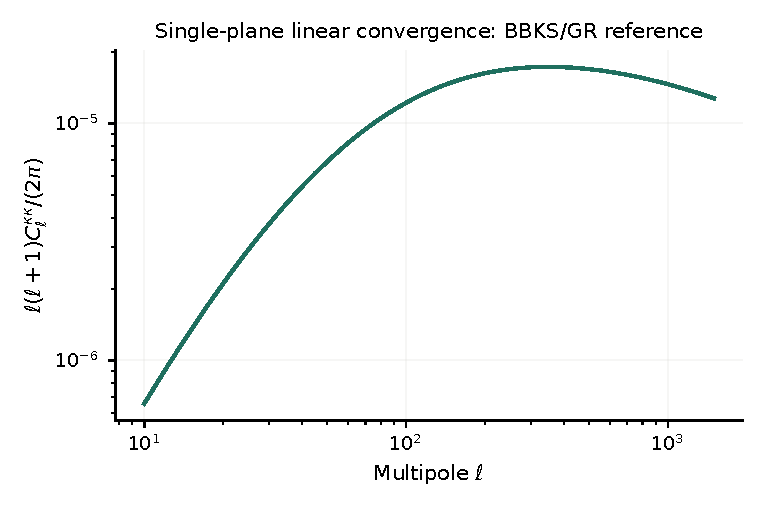
\includegraphics[width=.8\linewidth]{figures/linear_cosmic_shear_limber.pdf}
\caption{Angular convergence power for a source plane at $z_s=1$, evaluated with the linear GR growth and smooth transfer of the reference model. The displayed quantity is $\ell(\ell+1)C_\ell^{\kappa\kappa}/(2\pi)$.}\label{fig:angular-convergence}
\end{figure}

\subsubsection{Metric-response consistency test}
The general weak-field deflection probes the sum of the potentials with the $1/c^2$ convention given above. Equation~\eqref{eq:clkk} adopts the GR response $\Phi=\Psi$. A general scalar response enters the same observable through the density-to-Weyl transfer in Eq.~\eqref{eq:weyl-limber-corrected}.

\subsection{Growth, slip and the velocity--lensing ratio}
\label{sec:metric-scalar-joint}
Cosmological scalar perturbations probe an additional sector of the metric response. At subhorizon scales, in the quasistatic regime and in a specified gauge, a minimally useful parameterization of the scalar response is
\begin{align}
-k^2\Psi&=4\pi G a^2\bar\rho_m\,\mu(k,a)\,\delta_m,\\
\Phi&=\eta(k,a)\Psi,\qquad
\Sigma(k,a)=\frac{\mu(k,a)[1+\eta(k,a)]}{2}.
\end{align}
The single field $\Psi$ controls nonrelativistic acceleration, whereas $\Phi+\Psi$ controls weak and strong lensing. In the general-relativistic limit $\mu=\eta=\Sigma=1$. In the QICT description, $\mu$ and $\eta$ are defined by the scalar density and metric kernels of the same renormalized state used for the tensor response.

For pressureless matter, negligible anisotropic stress in the matter sector and a quasistatic conserved fluid, the continuity and Euler equations give
\begin{equation}
D_k''+\left(2+\frac{H'}{H}\right)D_k'-\frac32\Omega_m(a)\mu(k,a)D_k=0,
\qquad {}'=\frac{\dd}{\dd\ln a}.
\label{eq:joint-growth}
\end{equation}
For physical peculiar velocity $\mathbf v_m$ and comoving gradient $\nabla$, define $\theta_m=\nabla\cdot\mathbf v_m/(aH)$. With $f=D_k'/D_k$, the linear continuity relation gives $\theta_m=-f\delta_m$. The ideal velocity--lensing statistic obeys \cite{Zhang07}
\begin{equation}
\boxed{E_G(k,z)=\frac{\Omega_{m0}\,\Sigma(k,z)}{f(k,z)}.}\label{eq:eg-null}
\end{equation}
The relation follows from $-k^2(\Phi+\Psi)=3H_0^2\Omega_{m0}\Sigma\delta_m/a$, together with the continuity relation, after common normalization factors have been removed. It is independent of the matter-power amplitude in the idealized deterministic, scale-matched limit. Galaxy bias, redshift-space distortions, nonlinear contributions and observational window functions enter the covariance and window of a measured estimator.

The baseline $\Omega_{m0}=0.315$ yields $f(0.5)=0.76087$ and $E_G(0.5)=0.41400$ from a direct integration of Eq.~\eqref{eq:joint-growth}. For an explicit alternative scalar-response \emph{example}, $\mu=1.05$ and $\eta=0.90$ give $\Sigma=0.9975$, $f(0.5)=0.78363$ and $E_G(0.5)=0.40097$. If both growth histories have the same density amplitude at $a=0.01$ (and their growing matter-era solutions are separately imposed), the equal-time three-dimensional Weyl-potential power at $z=0.5$ changes by a factor $1.2683337$. The angular convergence spectrum instead integrates the changed growth along the line of sight. For a source plane at $z_s=1$, the ratios $C_\ell^{\kappa\kappa}(\mu=1.05,\eta=0.90)/C_\ell^{\kappa\kappa}(\mathrm{GR})$ are $1.2737472$, $1.2709505$ and $1.2695077$ at $\ell=50,200,1000$, respectively. Both use the same initial density amplitude at $a=0.01$ and the same background geometry. This exercise shows how a near-standard lensing strength can coexist with a different growth history. The values of $\mu$ and $\eta$ are selected inputs to this response test. The full calculation and normalization convention appear in the attached script.


\subsection{Direct inversion of the scalar response}
\label{sec:growth-inversion}
The growth equation and the velocity--lensing ratio also determine an inverse relation. At fixed wavenumber, assume conserved pressureless matter, a specified background $H(a)$ and $\Omega_{m0}$, the quasistatic scalar response of Eq.~\eqref{eq:joint-growth}, and $f\neq0$, $\mu\neq0$. Then
\begin{equation}\label{eq:growth-inversion}
\boxed{\begin{aligned}
\mu(k,a)&=\frac{2}{3\Omega_m(a)}
\left[f'+f^2+\left(2+\frac{H'}H\right)f\right],\\
\eta(k,a)&=\frac{2f(k,a)E_G(k,a)}{\Omega_{m0}\mu(k,a)}-1.
\end{aligned}}
\end{equation}
For the first identity, divide the growth equation by $D$ and use $D''/D=f'+f^2$. The second follows by substituting $\Sigma=\mu(1+\eta)/2$ into Eq.~\eqref{eq:eg-null}. An overall normalization of $D$ cancels from both expressions. In a numerical check, differentiating independently integrated growth histories recovers $(\mu,\eta)=(1,1)$ and $(1.05,0.90)$ with absolute errors below $2\times10^{-10}$. These are tests of the inversion under its stated assumptions. An observational application supplies the covariance of the reconstructed derivative, the background and the scale-matched velocity--lensing statistic.
